%Some d^i and s^i fixed to d_i and s_i.
%Rhetorical questions are okay in spoken lectures but I think they should be used more sparingly in text.

\section{Simplices, more about homology}
Previously we introduced the standard $n$-simplex $\Delta^n\subseteq\mathbf{R}^{n+1}$. Singular simplices in a space $X$ are maps $\sigma\colon\Delta^n\to X$ and constitute the set $\Sin_n(X)$. For example, $\Sin_0(X)$ consists of points of $X$. In addition to the \emph{face maps} $d_i\colon\Sin_n(X)\to\Sin_{n-1}(X)$ we described, there are also \emph{degeneracy maps} $s_i\colon\Sin_n(X)\to\Sin_{n+1}(X)$, and the collection $\{\Sin_n(X),d_i,s_i\}$ forms a \emph{simplicial set}. Simplicial sets are combinatorial models for topological spaces. In the language of category theory, which we will discuss shortly, we have a functor $\mathbf{Top}\to\{\text{simplicial sets}\}$.

To the semi-simplicial set $\{\Sin_n(X),d_i\}$ we then applied the free abelian group functor, obtaining a semi-simplicial abelian group. Using the $d_i$s, we constructed a boundary map $\partial$ which makes $S_\ast(X)$ a \emph{chain complex} because $\partial^2=0$ (see Exercise \ref{exer:simplicialidentities}). We capture this process in a diagram:
\begin{equation*}
\xymatrix{\mathbf{Top}\ar[d]\ar[r] & \{\text{semi-simplicial sets}\}\ar[r] & \{\text{semi-simplicial abelian groups}\}\ar[d]\\
    \{\text{simplicial sets}\}\ar[ur] & & \{\text{chain complexes}\}\ar[d]^{\text{take homology}}\\
 & &\{\text{graded abelian group}\}}
\end{equation*}
Given a chain complex $\partial\colon A_n\to A_{n-1}$, one can define its homology $H_n(A,\partial)=\ker\partial_n/\img\partial_n$.

Here's an example. Suppose we have $\sigma\colon \Delta^1\to X$. Define $\phi\colon\Delta^1\to\Delta^1$ which sends $(t,1-t)\mapsto (1-t,t)$. Precomposing $\sigma$ with $\phi$ gives another singular simplex $\overline{\sigma}$ which reverses the orientation of $\sigma$. It is \textit{not} true that $\overline{\sigma}=-\sigma$ in $S_1(X)$.

However, we show that $\overline{\sigma}\equiv -\sigma\bmod B_1(X)$, meaning there is a $2$-chain in $X$ whose boundary is $\overline{\sigma}+\sigma$. If $d_0\sigma=d_1\sigma$ so that $\sigma\in Z_1(X)$, then $\overline{\sigma}$ and $-\sigma$ are homologous: $[\overline{\sigma}]=-[\sigma]$ in $ H_1(X)$.

\begin{figure}
	\centering
	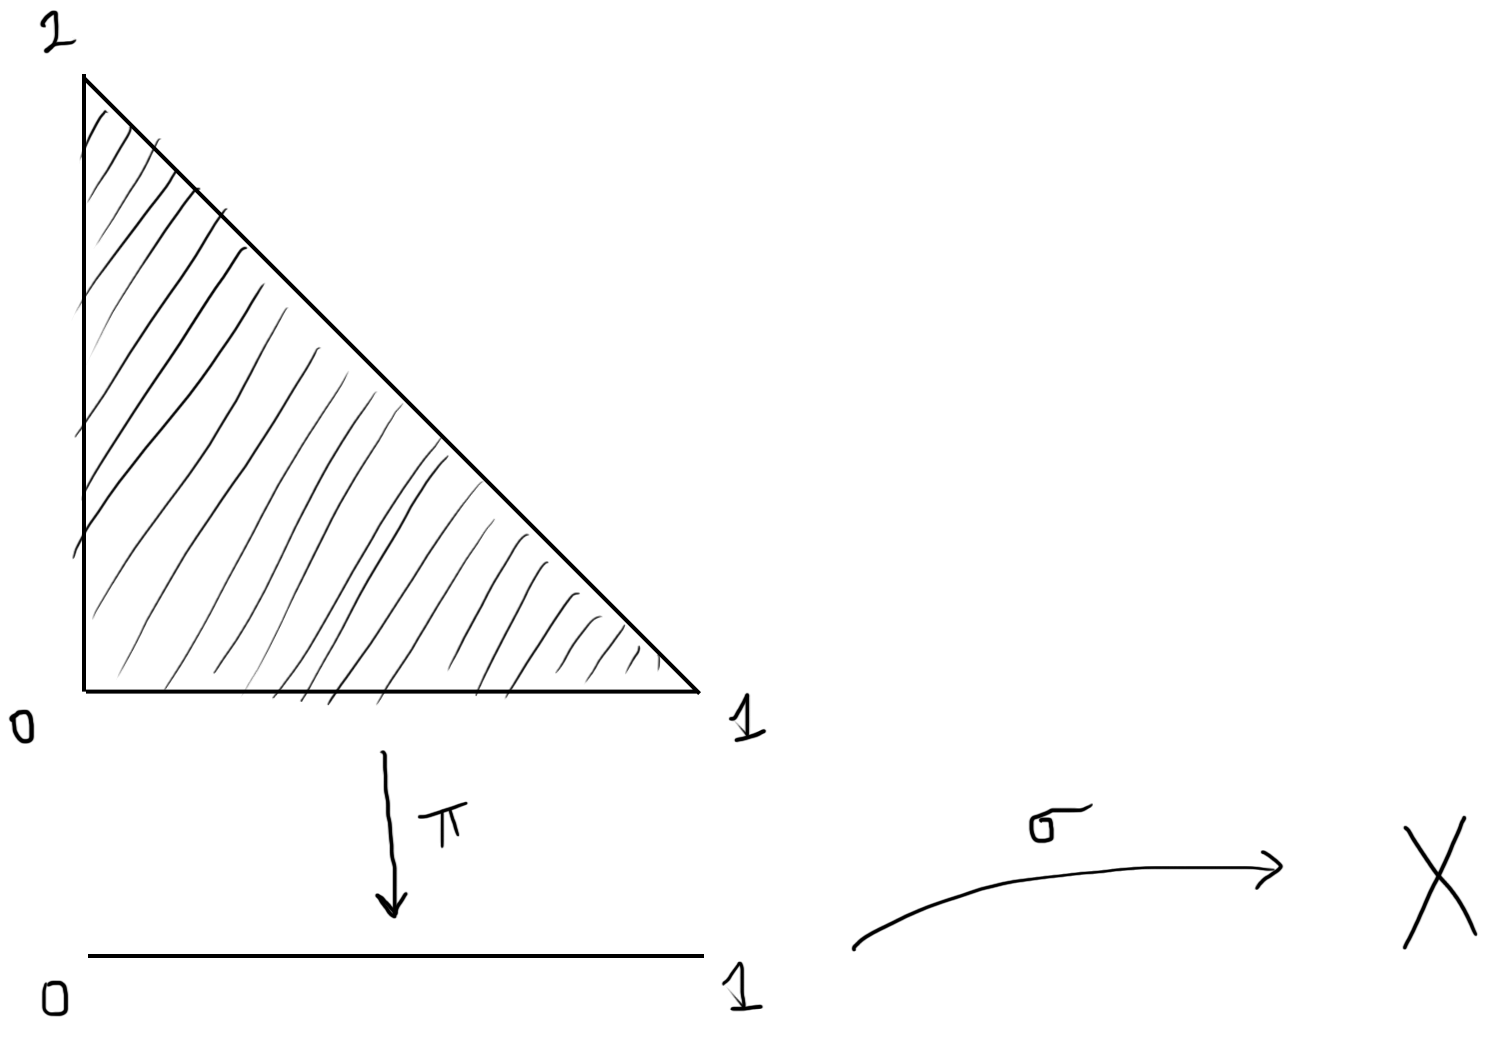
\includegraphics[width=0.6\linewidth]{assets/L02/02-pi-then-sigma}
	\caption{If $\sigma$ is a 1-simplex in $X$, then precomposing by $\pi$ gives a 2-simplex $\sigma \circ \pi$ in $X$.}
	\label{fig:02-pi-then-sigma}
\end{figure}

Let $c^n_{x}$ denote the constant $n$-simplex at $x$. Consider the 2-simplex in Figure \ref{fig:02-pi-then-sigma}. Its boundary is $\partial(\sigma\circ\pi)=\sigma\pi d^0-\sigma\pi d^1 +\sigma\pi d^2=\overline{\sigma}-c^1_{\sigma(0)}+\sigma$. To compensate for the unwanted $-c^1_{\sigma(0)}$ term, consider the constant $2$-simplex $c^2_{\sigma(0)}$; its boundary is $c^1_{\sigma(0)}-c^1_{\sigma(0)}+c^1_{\sigma(0)}=c^1_{\sigma(0)}$. So $\overline{\sigma}+\sigma=\partial(\sigma\circ\pi + c^2_{\sigma(0)})$ and $\overline{\sigma}\equiv -\sigma\bmod B_1(X)$ as claimed.

To give the simplest explicit examples, let's compute the homologies of $\emptyset$ and $\ast$. For the former, $\Sin_n(\emptyset)=\emptyset$, so $S_\ast(\emptyset)=0$. Hence $\cdots\to S_2\to S_1\to S_0$ is the zero chain complex. This means that $Z_\ast(\emptyset)=B_\ast(\emptyset)=0$. The homology in all dimensions is therefore $0$.

For $\ast$, we have $\Sin_n(\ast)=\{c^n_\ast\}$ for all $n\geq 0$. Consequently $S_n(\ast)=\mathbf{Z}$. The boundary maps $\partial\colon S_n(\ast)\to S_{n-1}(\ast)$ in the chain complex depend on the parity of $n$ as follows:
\[\partial(c^n_\ast)=\sum_{i=0}^{n}(-1)^i c^{n-1}_\ast=
\begin{cases}
    c^{n-1}_* & \text{for } n \text{ even, and}\\
    0 & \text{for } n \text{ odd.}
  \end{cases}
\]
This means that our chain complex is:
$$\cdots\to\mathbf{Z}\xrightarrow{0}\mathbf{Z}\xrightarrow{1}\mathbf{Z}\xrightarrow{0}\mathbf{Z}\to 0.$$
The boundaries coincide with the cycles except in dimension zero, where $B_0(\ast)=0$ while $Z_0(\ast)=\mathbf{Z}$. Therefore $ H_0(\ast)=\mathbf{Z}$ but $ H_i(\ast)=0$ for $i>0$.

We've defined homology groups for each space, but haven't considered what happens to maps between spaces. A continuous map $f\colon X\to Y$ induces a map $f_\ast\colon \Sin_n(X)\to\Sin_n(Y)$ by composition: $\sigma\mapsto f\circ \sigma=:f_\ast\sigma$. For $f_\ast$ to be a map of semi-simplicial sets, it needs to commute with face maps. Explicitly, we need $f_\ast \circ d_i = d_i \circ f_\ast$. A diagram is said to be \emph{commutative} if all composites with the same source and target are equal, so this is equivalent to commutativity of the below.
\begin{eqnarray*}
\xymatrix{\Sin_n(X)\ar[r]^{f_\ast}\ar[d]^{d_i} & \Sin_n(Y)\ar[d]^{d_i}\\
\Sin_{n-1}(X)\ar[r]^{f_\ast} & \Sin_{n-1}(Y)}
\end{eqnarray*}
We see that $d_if_\ast\sigma=(f_\ast\sigma)\circ d^i=f\circ\sigma\circ d^i$, and $f_\ast(d_i\sigma)=f_\ast(\sigma\circ d^i)=f\circ\sigma\circ d^i$ as desired. The diagram remains commutative when we pass to the free abelian groups of chains.

If $C_\ast$ and $D_\ast$ are chain complexes, a \emph{chain map} $f\colon C_\ast\to D_\ast$ is a collection of maps $f_n\colon C_n\to D_n$ such that the following diagram commutes for every $n$:
\begin{equation*}
    \xymatrix{
	C_n\ar[r]^{f_n}\ar[d]^{\partial_C} & D_n\ar[d]^{\partial_D}\\
	C_{n-1}\ar[r]^{f_{n-1}} & D_{n-1}
    }
\end{equation*}
For example, if $f\colon X\to Y$ is a continuous map, then $f_\ast \colon S_\ast(X)\to S_\ast(Y)$ is a chain map as discussed above.

A chain map induces a map in homology $f_\ast: H_n(C)\to H_n(D)$. The method of proof is a so-called ``diagram chase'' and it will be the first of many. We check that we get a map $Z_n(C)\to Z_n(D)$. Let $c\in Z_n(C)$, so that $\partial_C c = 0$. Then $\partial_D f_n(c) = f_{n-1}\partial_C c = f_{n-1}(0) = 0$, because $f$ is a chain map. This means that $f_n(c)$ is also an $n$-cycle, i.e., $f$ gives a map $Z_n(C)\to Z_n(D)$.

Similarly, we also get a map $B_n(C)\to B_n(D)$. Let $c\in B_n(C)$, so that there exists $c^\prime \in C_{n+1}$ such that $\partial_C c^\prime = c$. Then $f_n(c) = f_n\partial_C c^\prime = \partial_D f_{n+1}(c^\prime)$. Thus $f_n(c)$ is the boundary of $f_{n+1}(c^\prime)$, and $f$ gives a map $B_n(C)\to B_n(D)$.

The two maps $Z_n(C)\to Z_n(D)$ and $B_n(C)\to B_n(D)$ give a map on homology $f_\ast: H_n(X)\to H_n(Y)$, as desired.